\documentclass[thesis.tex]{subfiles}
\begin{document}
\chapter{Instantiating and Evaluating SecPAL}
\label{chap:apppal}

Mobile ecosystems contain a large number of entities interacting.
Devices interact with their users, as well as app stores, app developers, wireless access points, companies and networks.
Each entity has their own policies; some formal and described in documents such as the agreement between an app store and a developer.
Others are informal: a user may have preferences about which kinds of apps they want to install but may not go so far as to write these preferences down.
The ecosystem is distributed in nature with each entity not necessarily knowing about other entities until they interact, and with decisions made between entities rather than being delegated to an arbiter who enforces an overarching policy.

Formal languages are used to write such policies without ambiguity and describe precisely how decisions are made.
Translating policies into formal language allows us to compare different policies, preferences and rules in mobile ecosystems rigorously.
We can also use the formal policy to automate the policy enforcement process, if desired.

SecPAL is an authorization language designed by Becker et al{.} to make access control decisions in distributed systems~\cite{becker_secpal:_2010}.
In particular it was designed to be expressive, clear, intuitive, decidable and extensible.
The extensibility of SecPAL is especially important to us as we can apply the language to a new domain by instantiating it with predicates and constraints appropriate there.

\newcommand{\bnfcomment}[1]{\slshape{\color{gray} (#1)}}
\newcommand{\secpal}[1]{\texttt{#1}}
\begin{figure}\footnotesize
  \begin{tabular}{r r l c}
    e          & $\Coloneqq$ & \secpal{x}                                       & \bnfcomment{variables}         \\
               & $\vert$     & \secpal{A}                                       & \bnfcomment{constants}         \\
    pred       & $\Coloneqq$ & \secpal{has} $\vert$ \secpal{can} $\vert$ \dots  & \bnfcomment{predicates}        \\
    D          & $\Coloneqq$ & 0                                                & \bnfcomment{no delegation}     \\
               & $\vert$     & $\infty$                                         & \bnfcomment{delegation}        \\
    vp         & $\Coloneqq$ & pred e$_1$ \dots e$_n$                           & \bnfcomment{verb phrase}       \\
               & $\vert$     & \secpal{can-say}$_D$ fact                       \\
               & $\vert$     & \secpal{can-act-as}  e                          \\
    f          & $\Coloneqq$ & e vp                                             & \bnfcomment{fact}              \\
    claim      & $\Coloneqq$ & f \secpal{if} f$_1$,\dots, f$_n$; c             \\
    assert     & $\Coloneqq$ & e \secpal{says} claim.                          \\
    AC         & $\Coloneqq$ & assert$_1$ \dots assert$_n$                      & \bnfcomment{assertion context} \\
    c          & $\Coloneqq$ & $\top$                                           & \bnfcomment{no constraint}     \\
               & $\vert$     & e$^\prime_1 =$ e$^\prime_2$                      & \bnfcomment{constraints}       \\
               & $\vert$     & \dots                                           \\
    e$^\prime$ & $\Coloneqq$ & e $\vert$ function(e$_1$,\dots e$_n$)           \\


  \end{tabular}
  \caption{BNF description of SecPAL.}
\label{fig:secpal-grammar}
\end{figure}

\section{Why SecPAL}
\label{sec:why-apppal}

For modelling and writing policies I want to start from a policy
language that supported several key features; namely:

\begin{itemize}
  \item Model decisions at separate locations.  Mobile ecosystems are
    inherently distributed, and decisions made by one device may not be
    the same as the decisions made by another device.  They may, however
    wish to share information.  By opting for a distributed language we
    can check the policies locally and make a decision based on that
    user's information rather than by deferring to an all-seeing policy
    enforcer.  This suits the problem better because individual devices
    and stores have to make decisions on their own and may not have access
    to all known information.

  \item Calling external functions that can obtain extra information
    about entities that may require special actions to fetch: for example
    an explicit ``okay'' from the user, or some metadata about an app like
    its version number.  If I don't allow the ability to fetch this
    information on-the-fly then it will have to be requested before
    checking the policy.

    I also want to be able to use static analysis tools as part of
    our policies.  These tools can infer complex properties of apps, but
    the low-level details they check for needn't be expressable in our
    high level policies.  For example it is not necessary to encode how
    data moves over intents in AppPAL policies, but it is necessary to be
    able to say some app leaks information to another app.  A tool, such
    as FlowDroid can check for this, and there is no need to replicate the
    checking in AppPAL if I can simply call out to FlowDroid to give us a
    decision.

  \item Delegation.  I want to make a decision based on information from an
    external source.  This suggest that a \emph{can-say} mechanism is required
    b
    that will allow us to express how trust is distributed.   Since the
    relationship between app stores and devices is one where a user delegates
    trust to the store and the device uses the external store to obtain the app
    this would hint that being able to express delegation will allow us to write
    more accurate policies.
\end{itemize}

Additionally I also wanted a language that was readable and easy to extend; a stated goal of the SecPAL language~\cite{becker_secpal:_2010}.
SecPAL 
\todo{MORE! How did it meet my requirements? Why SecPAL over XACML/PolicyMaker/DKAL, for example}

\subsection{Comparison to XACML}
\todo{Make a comparison.  Show syntaxes, explain about XACML's semantics being poorly defined.}

An alternative to SecPAL might be XACML.
XACML is a powerful access control and policy language with a published standard~\cite{oasis_extensible_2013}.
From XACML version 3.0 XACML can express delegation relationships~\cite{oasis_xacml_2010}.

XACML does not have well defined semantics.
The standards that describe the language are expressed in natural language, and are notoriously difficult to interpret\todo{CITATION}.
There have been several attempts to describe XACML's semantics formally~\cite{ramli_xacml_2012,ramli_logic_2014,bryans_reasoning_2005}.
These help define XACML better but, the complexity of the language and the lack of a single accepted formal semantics make it less attractive.
In contrast SecPAL's semantics are given by Becker with the description of the language.

\begin{figure}\centering
  \begin{tabular}{l p{0.7\linewidth}}
    \toprule
    $AC,\theta \vdash q$                     & Defining relation. A query assertion $q$ is valid given the assertions contained in the assertion context $AC$ and a variable substitution $\theta$. \\
    $\epsilon$                               & The empty substitution.                                                                                                                              \\
    \midrule
    $AC,\theta \vdash e \text{ says } fact$  & if $AC,\infty \models e\theta \text{ says } fact\theta$ and $dom(\theta) \subseteq vars(e \text{ says } fact)$                                       \\
    $AC,\theta_1\theta_2 \vdash q_1, q_2$    & if $AC,\theta_1 \vdash q_1$ and $AC,\theta_2 \vdash_2 q_2\theta_1$                                                                                   \\
    $AC,\theta \vdash q_1 \text{ or } q_2$   & if $AC,\theta \vdash q_1$ or $AC,\theta \vdash q_2$                                                                                                  \\
    $AC,\epsilon \vdash \mathsf{not}(q)$     & if $AC,\epsilon \not\vdash q$ and $vars(q) = \emptyset$                                                                                              \\
    $AC,\epsilon \vdash c$                   & if $\models c$                                                                                                                                       \\
    \bottomrule                             \\
  \end{tabular}
  \caption[SecPAL's semantics.]{SecPAL's semantics as described by Becker~\cite{becker_secpal:_2010}.}
\end{figure}

The complexity of XACML is not helped by its syntax which makes it difficult to read.
XACML policies are verbose, and written in XML.
To help developers write policies alternative notations are available that compile into XACML's XML notation.
ALFA is one such version that is maintained by the XACML developers\footnote{Prior to 2014 it was maintained by Axiomatics.}~\cite{oasis_xacml_technical_comitee_abbreviated_????}, however many other's exist including graphical languages~\cite{henrik_nergaard_scratch-based_2015}, languages based off propositional logic~\cite{zhang_synthesising_2004} and answer set programming~\cite{ramli_xacml_2012}.
In contrast SecPAL is designed for readability, and so avoids the need for wrapper languages to simplify it.

\section{Instantiating SecPAL for mobile ecosystems}
\label{sec:instantiating}

SecPAL is a generic language.
In SecPAL's grammar~(\autoref{fig:secpal-grammar}) predicates and constraint functions that describe the decisions and checks done in a particular domain.
The choice of predicates and constraints defines the decisions an \emph{instantiation} of SecPAL can talk about.
In past work SecPAL has been instantiated for many other domains.
Humphrey~\etal instantiated SecPAL with predicates for the GridFTP protocol to create a Grid access control policy language~\cite{humphrey_fine-grained_2007}.
Aziz~\etal created SecPAL4DSA by adding predicates for data-sharing agreements~\cite{aziz_secpal4dsa:_2011}.
Becker~\etal added predicates for describing \ac{PII}-handling preferences and created SecPAL4P~\cite{becker_framework_2009}

To describe policies in mobile ecosystems I developed an instantiation of SecPAL called AppPAL~\cite{hallett_apppal_2016}.
AppPAL was initially focussed on describing app installation policies, however it was later extended further to describe SP4BYOD---a framework for describing BYOD policies using SecPAL.
To further explore these areas an implementation of SecPAL was created and is described in \autoref{sec:implementation}.

\subsection{Predicate Conventions}
\label{ssec:types}

\newcommand{\descPred}[2]{\emph{subject} \texttt{\textbf{#1}\emph{#2}}}
\begin{table}
  \begin{tabular}{l l}
    \toprule
    Prefix                      & Meaning                                            \\
    \midrule
    \descPred{can}{Action}      & The subject is allowed to perform the action.      \\
    \descPred{has}{Action}      & The subject has performed the action.              \\
    \descPred{is}{Property}     & The property holds true for the subject.           \\
    \descPred{must}{Obligation} & The subject is required to satisfy the obligation. \\
    \bottomrule
  \end{tabular}
  \caption{Standard prefixes used for AppPAL predicates.}
  \label{tab:predicate-prefixes}
\end{table}

When instantiating SecPAL we use predicates based on four verbs: \emph{can}, \emph{has}, \emph{is} and \emph{must}.
These verbs describe facts common in many different policies.
An \emph{is} predicate is used to restrict variables to a given type.
An \emph{can} predicate is used to describe permissible actions.
For example in a \ac{BYOD} policy a company might describe what apps a device can install, and what company data a user can access.
A user might have a privacy preference describing what parts of their personal data an app can share.
App stores have procedures to go through before a developer can submit an app. \todo{CITE}
When we need to describe the conditions for an action going ahead we use the can statement.

\begin{description}
\item[\bfseries\texttt{subject \emph{is}Type}]
  A typing statement.  The \emph{subject} is an example of the \emph{type}.  An
  example might be that \lstinline!'anrgry-birds' isApp! or that
  \lstinline!'jennie' isEmployee!.
\item[\bfseries\texttt{subject \emph{has}Action}]
  A statement of action.  The \emph{subject} has carried out an \emph{action} in
  the past. For example if an app has requested a permission then we write
  \lstinline!App:A hasRequestedPermission(Permission:P)!, if a device requires
  its owner to grant a permission we might write
  \begin{lstlisting}
'device' says User:U can-say
  App:A hasBeenGranted(Permission:P)
  if 'device' isOwnedBy(U).
  \end{lstlisting}
\item[\bfseries\texttt{subject \emph{can}Action}]
  An authorization. The \emph{subject} is permitted to carry out the \emph{action}.
  For example \lstinline!Device:D canInstall(App:A)! to say what apps a device
  can install or \lstinline!App:A canConnectTo(URL:U)! to describe a limitation
  on app network abilities.
\item[\bfseries\texttt{subject \emph{must}Action}]
  An obligation.  The \emph{subject} should carry out the \emph{action} as soon
  as possible.
  An example might be requiring the device inform a company's IT department if
  there have been three unsuccessful password attempts:
  \begin{lstlisting}
'company' says Device:D mustInform('it', 'login-failure')
  if D hasUnsuccesfulLogins(N)
  where N >= 3.
  \end{lstlisting}
\end{description}

This differs slightly from the approach taken with the SecPAL4P and SecPAL4DSA~\cite{becker_framework_2009,aziz_secpal4dsa:_2011} instantiations.
Both these languages add additional special phrases to SecPAL's grammar.
For example SecPAL4P adds a \emph{may} and \emph{will} phrase to describe whether a behavior could or will be carried out.
If Alice, a policy author, wished to use SecPAL4P to say that someone can forget her email address she could write:\footnote{%
Example taken from~\cite{becker_framework_2009}  SecPAL4P also has relaxed safety rules, that permit the variables $x$ and $t$ to be in the head of the rule, but not the body.}
\begin{lstlisting}
Alice says x may delete Email within t
\end{lstlisting}
An analogous AppPAL rule would be:
\begin{lstlisting}
'alice' says User:X canDeleteWithin('email', Time:t)
  where currentTime() < t.
\end{lstlisting}
The AppPAL is arguably slightly less succinct, but more explicit than the SecPAL4DSA.


\subsection{Type Notation}

When writing a policy it is common to use conditions in facts that limit the scope of a variable.
To do this we use \emph{is}-predicates, that give their subject a type.
For example \emph{Alice} might declare that \emph{Bob} is responsible for saying which apps she can install.
This can be written in SecPAL as follows:
\begin{lstlisting}
'alice' says 'bob' can-say App isInstallable
  if App isApp.
\end{lstlisting}
When writing this we added a condition \lstinline{if App isApp}, that Bob can only talk about Apps as being installable.
Generalising this pattern we use predicates starting with \emph{is} to give types to their subjects.
If a policy rule contains a lot of variables, however these typing conditions can become very verbose. 
To simplify the policy rules, AppPAL adds a sugared notation for typing statements by extending SecPAL's grammar for variables:

{
  \newcommand{\nonterminal}[1]{$\langle$#1$\rangle$}
  \newcommand{\terminal}[1]{\textbf{#1}}
  \begin{tabular}{r c l}
    \footnotesize
    \nonterminal{E}         & $\Coloneqq$ & \nonterminal{Variable} $\vert$ \terminal{'constant'} \\
    \nonterminal{Variable}  & $\coloneqq$ & \new{\terminal{Type}\terminal{:}\terminal{Var}} $\vert$ \terminal{Var}
  \end{tabular}
}

Expand the AppPAL types into SecPAL conditions is described in \autoref{lst:type-expansion}.
This is run when parsing AppPAL code, and adds a semantic rule to AppPAL
  that if a variable in the head of an assertion has a type
  then it is removed and a condition that the variable is that type is added to the body of the assertion. 
If a variable in the body of an assertion has a type then it is an error.

\begin{lstlisting}[language=Python, float, caption={Procedure used to expand types from AppPAL into SecPAL.}, label={lst:type-expansion}]
def expand_types(a: Assertion) -> Assertion:
  for v in a.head.vars():
    if v.type != None:
      f = Fact(v, 'is'++str(v.type))
      a.body.add(f)
  return a
\end{lstlisting}

Using this sugared notation, the earlier example becomes:
\begin{lstlisting}
'alice' says 'bob' can-say App:A isInstallable
\end{lstlisting}

For a more complex example consider the following example taken from a BYOD policy.
\begin{lstlisting}
'company' says Device:D canConnectToAP(AP:X) 
  if X isOwnedByCompany.
\end{lstlisting}
The rule states that the company will only allow devices to connect to company owned access points.
The syntactic sugar is expanded into following equivalent policy.
\begin{lstlisting}
'company' says Device canConnectToAP(X) 
  if X isOwnedByCompany,
     Device isDevice,
     X isAP.
\end{lstlisting}
I feel the first is easier to read.
It also avoids hiding the condition that the access point must be company owned amongst typing statements aiding readability.


\section{Examples of AppPAL}

Consider the following example: a user, Alice, may have rules she has to follow
when using apps for work and her own policies when using apps at home in her
private life. Using AppPAL I can write policies for work and home, and decide
which policy to enforce using a user's location, or the time of day:

\begin{lstlisting}
'alice' says App isRunnable
  if 'home-policy' isMetBy(App)
  where at('work') = false.

'alice' says App isRunnable
  if 'work-policy' isMetBy(App)
  where beforeHourOfDay('17') = true.
\end{lstlisting}

I can delegate policy specification to third parties or roles, and assign principals to roles:

\begin{lstlisting}
'alice' says 'it-department' can-say 'work-policy' isMetBy(App).
'alice' says 'alice' can-act-as 'it-department'.
\end{lstlisting}

I can write policies specifying which permissions an app must or must not have
by its app store categorization. For example, it would be okay allowing a
photography app access to the camera, but not to allow access to location data
if the user doesn't want their photos geotagged.

\begin{lstlisting}
'alice' says App isRunnable
  if 'permissions-policy' isMetBy(App).
'alice' says 'permissions-policy' isMetBy(App)
  if App isAnApp
  where
    category(App, 'Photography'),
    hasPermission(App, 'LOCATION') = false,
    hasPermission(App, 'CAMERA') = true.
\end{lstlisting}

\section{Implementation}
\label{sec:implementation}

AppPAL is implemented as a library.
The library is used to create an instance of AppPAL that is given one or more policies to enforce (\autoref{fig:apppal-inputs-outputs}).
The instance can be queried and will give decisions based on whether the queried assertion is valid according to the policy.
As part of the constraint checking AppPAL can also be connected to external databases, systems, and static analysis tools.
These can provide AppPAL with additional information external to that provided by SecPAL at the time of checking.

Implementing AppPAL as a library allows it to be embedded into a variety of situations.
It can be part of an app store checking the apps sold against a policy.
It can be used on a device (AppPAL is written in Java, and minimal changes are needed to let it run on Android), checking apps before they are installed by the package manager.
There is also a command-line tool which is useful for testing and modelling policies.

The AppPAL interpreter implements SecPAL's evaluation rules (shown in~\autoref{fig:secpal-rules}) directly.
This differs from Becker's original description of SecPAL~\cite{becker_secpal:_2010} which describes evaluation through Datalog$^C$.
Datalog$^C$ is a version of Datalog with support for constraints~\cite{li_datalog_2003}.
Rather than implementing Datalog$^C$ and then AppPAL atop it (we could not find an existing implementation), AppPAL implements the evaluation rules directly.
This allows greater control over when AppPAL caches results, which is important in memory-constrained mobile devices.

\begin{figure}
  \centering
  \begin{eqnarray*}
    \infer[\textsf{\scriptsize cond}]{%
      AC, D \models A\textsf{~says~}fact\theta
    }{%
      \begin{array}[c]{c}
        \left(A\textsf{~says~}\textit{fact}\textsf{~if~}\textit{fact}_1, \ldots, \textit{fact}_k, c\right) \in AC \\
        AC,D\models A\textsf{~says~}\textit{fact}_i\theta \; \forall i \in \{1\cdots k\}
      \end{array}
      & \models{c\theta}
      & \textsf{vars}(\textit{fact}\theta) = \emptyset)
    }\\
    \infer[\textsf{\scriptsize can say}]{%
      AC, \infty \models A\textsf{~says~}\textit{fact}
    }{%
      AC, \infty \models A\textsf{~says~}B\textsf{~can~say}_D \textit{fact}
      & AC, D \models B\textsf{~says~}\textit{fact}
    } \\
    \infer[\textsf{\scriptsize can act as}]{%
      AC, D \models A\textsf{~says~}B~\textit{verbphrase}
    }{%
      AC, D \models A\textsf{~says~}B\textsf{~can~act~as~}C
      & AC, D \models A\textsf{~says~}C~\textit{verbphrase}
    }
  \end{eqnarray*}
  \caption[Inference rules used to evaluate {SecPAL}.]{The inference rules used to evaluate {SecPAL}. All {SecPAL} rules are
  evaluated in the context of a set of other assertions $AC$ as well as an
  allowed level of delegation $D$ which may be $0$ or $\infty$.}
\label{fig:secpal-rules}
\end{figure}

\begin{figure}
  \centering
  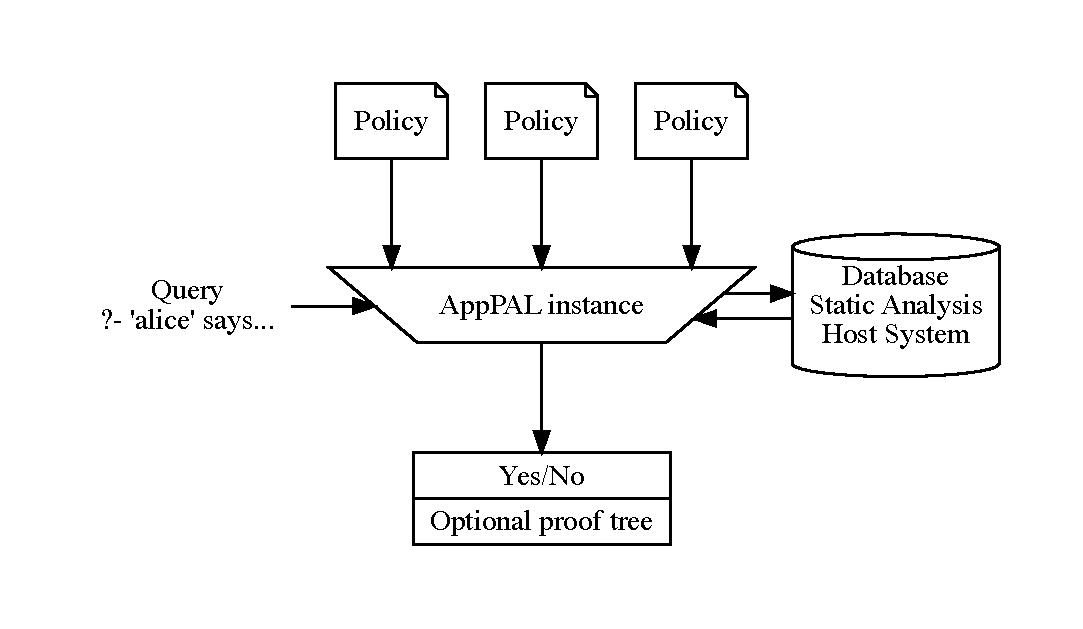
\includegraphics[width=\linewidth]{figures/apppal-evaluation.pdf}
  \caption{AppPAL's inputs and outputs}
  \label{fig:apppal-inputs-outputs}
\end{figure}

\subsection{Evaluation}
\label{ssec:evaluation-alg}

To make queries against a policy AppPAL is first given one or more policy files.
These are parsed, and the assertions within them are added to the \ac{AC}.
The AC is then preprocessed to extract additional information; summarized in \autoref{tab:apppal-sets}.
If a constant is used before a \emph{says} statement, or it is used as the subject of a \emph{can-say} fact then the constant is marked as \emph{voiced}.
If the constant is used immediately after the \emph{says} or as the subject of a fact then it is marked as a \emph{subject}.
The predicates used in the policy are also extracted and marked as \emph{derivable}.
This allows some queries to be decided automatically and some rules to be flagged as unusable in the assertion context.
If a rule relies on un-Derivable predicates then it cannot be used to make decisions.

A results table is also created.
All ground facts in the assertion context are added to the results table as they are known to be true.
The table stores partial results and previously established proofs.
The table is indexed by queries and a delegation depth, partial results (i.e. that a query is being evaluated).
This allows previous results to reused without re-computation or constraint re-evaluation.
It also prevents AppPAL proofs growing infinite in size (and the decision process not terminating).
If when searching for a proof we encounter a query that we are currently evaluating, i.e.~one that exists higher in the current proof tree, we treat it as false. 
This results table is shared between evaluations of an \ac{AC}.

\begin{table}
  \centering
  \newcommand{\myset}[1]{\ensuremath{\text{\sffamily #1}}}
  \begin{tabular}{r l c}
    \toprule
    $c \in \myset{Voiced} \impliedby$     & $\exists \left(c \text{~says~} \cdots\right) \in \text{AC}$                        & $\bigvee$ \\
                                          & $\exists \left(\star \text{~says~} c \text{~can-say~} \cdots\right) \in \text{AC}$ &           \\
    $c \in \myset{Subjects} \impliedby$   & $\exists \left(\star \text{~says~} c\cdots\right) \in \text{AC}$                   & $\bigvee$ \\
                                          & $\exists \left(\cdots \text{~if~} \cdots,c~\star,\cdots\right) \in \text{AC},$     &           \\
                                          & $c \in \myset{Constants}$                                                          &           \\
    $p \in \myset{Derivable} \impliedby$  & $\exists \left( \cdots \star~p\left(\cdots\right) \cdots\right) \in \text{AC}$     &           \\
    \bottomrule                          \\
  \end{tabular}
  \caption{Sets used in AppPAL evaluation.}
  \label{tab:apppal-sets}
\end{table}

\SetKwProg{Fn}{}{\string:}{}
\SetKwIF{If}{ElseIf}{Else}{if}{:}{elif}{else:}{}
\SetKwFunction{FnEvaluate}{Evaluate}
\SetKwFunction{FnContains}{Contains}
\SetKwFunction{FnCheckConstraint}{Check Constraint}
\SetKwFunction{FnCheckBody}{Check Body}
\SetKwFunction{FnGet}{Get}
\SetKwFunction{FnSet}{Set}
\SetKwFunction{FnCond}{Cond}
\SetKwFunction{FnConstraint}{Constraint}
\SetKwFunction{FnCanSay}{CanSay}
\SetKwFunction{FnCanActAs}{CanActAs}
\SetKwFunction{FnCanSayCanActAs}{CanSay-CanActAs}
\SetKwFunction{FnValid}{Is Valid?}
\SetKwFunction{FnVarSubs}{Variable Substitutions}
\SetKwFunction{FnAssertions}{Assertions}
\SetKwFunction{FnConstants}{Constants}
\SetKwFunction{FnSpeakers}{Speakers}
\SetKwFunction{FnSubjects}{Subjects}
\SetKwFunction{FnConstants}{Constants}
\SetKwFunction{FnUnify}{Unify}
\SetKwFunction{FnHead}{Head}
\SetKwFunction{FnApply}{Apply}
\SetKwFunction{FnBody}{Body}
\SetKwFunction{FnVariables}{Variables}
\begin{algorithm}
  \Fn(){\FnEvaluate{AC, Results Table, Query, D}}{
    \If{Results Table.\FnContains{(Query, D)}}{
      \Return{Results Table.\FnGet{(Query, D)}}\;
    }
    \Else{
      p $\gets$ \FnCond{AC, Results Table, Query, D}\;
      \If{p.\FnValid{}}{
        Results Table.\FnSet{(Query, D), (Proven, p)}\;
        \Return{(Proven, p)}\;
      }
      \Else{
        p $\gets$ \FnCanSayCanActAs{AC, Results Table, Query, D}\;
        \If{p.\FnValid{}}{
          Results Table.\FnSet{(Query, D), (Proven, p)}\;
          \Return{(Proven, p)}\;
        }
        \Else{
          Results Table.\FnSet{(Query, D), Failure}\;
          \Return{Failure}\;
        }
      }
    }
  }
    \caption{Pseudocode for evaluating a query.}
\end{algorithm}
\begin{algorithm}
  \ContinuedFloat
  \Fn(){\FnCond{AC, Results Table, Query, D}}{
    \For{a $\in$ \FnAssertions{AC}}{
      u $\gets$ Query.\FnUnify{a.\FnHead{}}\;
      \If{u.\FnValid{}}{
        a $\gets$ a.\FnApply{u} 
        \If{\FnVariables{a} = $\emptyset$}{
          \Return{\FnCheckBody{AC, Results Table, a, D}}
        }
      }
    }
    \Return{Failure}
  }
    \caption{Pseudocode for using the cond-rule.}
\end{algorithm}
\begin{algorithm}
  \ContinuedFloat
  \Fn(){\FnCanSayCanActAs{AC, Results Table, Query, D}}{
    \For{c $\in$ \FnConstants{AC}}{
      \If{c $\in$ \FnSubjects{AC}}{
        p $\gets$ \FnCanActAs{AC, Results Table, Query, D}\;
        \If{p.\FnValid{}}{\Return p}
      }
      \If{c $\in$ \FnSpeakers{AC}}{
        p $\gets$ \FnCanSay{AC, Results Table, Query, D}\;
        \If{p.\FnValid{}}{\Return p}
      }
    }
    \Return{Failure}
  }
  \caption{Pseudocode for using the can-say and can-act-as rules.}
\end{algorithm}
\begin{algorithm}
  \ContinuedFloat
  \Fn(){\FnCheckBody{AC, Results Table, Assertion, D}}{
    \For{$\theta \in$ \FnVarSubs{AC, Assertion}}{
      a $\gets$ Assertion.\FnApply{$\theta$}\;
      \If{$\forall$ b $\in$ a.\FnBody{}: \FnEvaluate{AC, Results Table, b, D}.\FnValid{}}{
        p $\gets$ \FnCheckConstraint{a.\FnConstraint{}}\;
        \If{p.\FnValid{}}{\Return{p}}
      }
    }
    \Return{Failure}
  }
  \caption{Pseudocode for evaluating the body of an assertion, used by the cond-rule.}
\end{algorithm}



\subsection{Correctness}
\todo{You know you're going to have to do this.}
\subsection{Benchmarks}
\label{ssec:benchmarks}

If AppPAL were to run on a mobile phone, apps should be checked as they are installed.
Since policy checks may involve inspecting many rules and constraints one may ask whether the checking will be acceptably fast.
Downloading and installing an app takes about 30 seconds on a typical Android phone over Wifi.
If checking a policy delays this even further a user may become annoyed and disable AppPAL.

To give a measure the performance of AppPAL a synthetic benchmark was developed.
The policy checking procedure is at its slowest when having to delegate repeatedly;
the depth of the delegation tree is the biggest factor for slowing the search.
Synthetic benchmarks were created to check that the checking procedure performed acceptably.
Each benchmark consisted of a chain of delegations.
The \emph{1 to 1} benchmark consists of a repeated delegation between all the principals.
In the \emph{1 to 2} benchmark each principal delegated to 2 others and in the \emph{1 to 3} benchmark each principal delegated to 3 others.
These benchmarks are reasonable as they model the slowest kinds of policies to
evaluate---though worse ones could be designed by delegating even more or triggering an expensive constraint check.

For each benchmark we controlled the number of principals in the policy file:
as the number of principals increased so did the size of the policy.
The results are shown in \autoref{tab:benchmarks}.
Most typical policies (such as those discussed in \autoref{chap:apps-and-stores} and \autoref{chap:byod}), use only few delegations per decision.
I believe the policy checking performance of AppPAL is acceptable as unless a policy consists of hundreds of delegating principals the overhead of checking an AppPAL policy is negligible, even on a power constrained device such as a mobile phone.

\begin{table}
  \centering\sffamily
    \begin{tabular}{c c r@{.}l}
      \toprule
      Delegations & Principals & \multicolumn{2}{c}{Time (s)} \\
      \midrule
      1 to 1 & 10   &  0&01 \\
      1 to 1 & 100  &  1&00 \\
      1 to 1 & 500  & 20&90 \\
      1 to 1 & 1000 & 88&73 \\
      \midrule
      1 to 2 & 10   &  0&01 \\
      1 to 2 & 100  &  0&43 \\
      1 to 2 & 500  &  7&36 \\
      1 to 2 & 1000 & 27&47 \\
      \midrule
      1 to 3 & 10   &  0&01 \\
      1 to 3 & 100  &  0&24 \\
      1 to 3 & 500  &  3&99 \\
      1 to 3 & 1000 & 15&28 \\
      \bottomrule
    \end{tabular}
    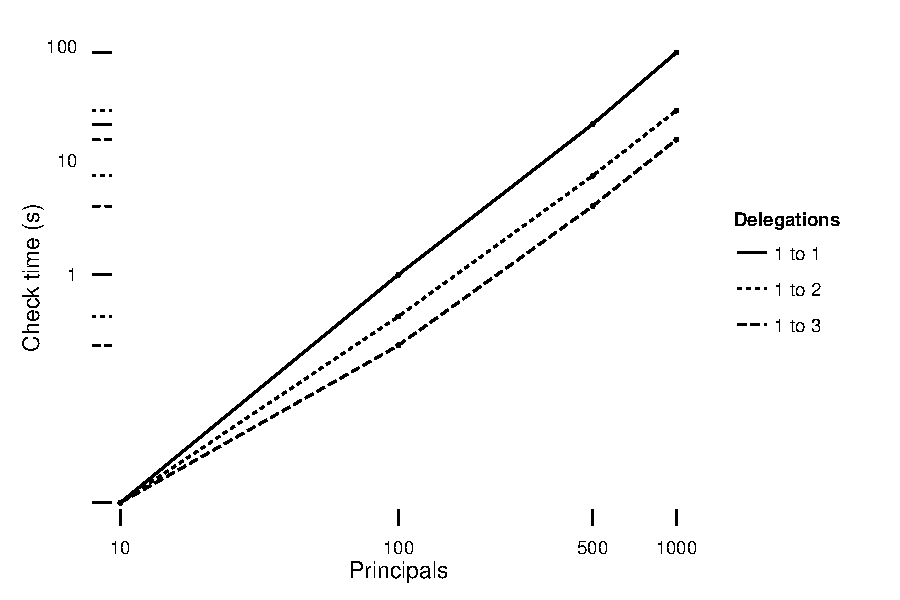
\includegraphics[width=0.70\linewidth]{figures/benchmarks.pdf}
  \caption{Benchmarking results on a Nexus 4 Android phone.}
  \label{tab:benchmarks}
\end{table}

\end{document}

%%% Local Variables:
%%% mode: latex
%%% TeX-master: "../thesis"
%%% End:
